\section{Binomial Theorem}

\begin{theorem}[Binomial Theorem]
    For any $x \in \R$, for any $n \geq 0$ natural number
    $$
    (1+x)^n = \sum_{k=0}^n \binom{n}{k} x^k
    $$
\end{theorem}

\begin{proof}
    $$
    \text{LHS} = (1+x)^n = \underbrace{(1+x) (1+x) \cdots (1+x)}_{\text{$n$ times}}
    $$
    When we expand and collect the like terms, we get a polynomial of the form
    $$
    \sum_{k=0}^n c_k x^k = c_0 + c_1x + c_2 x^2 + \cdots + c_n x^n
    $$
    For $k$, the only way to get $x^k$ in the expansion of the LHS is if for $k$ of the $n$ terms in the product to contribute to to $x$, and the rest $n-k$ of the terms to contribute to $1$.

    In total, we have $\binom{n}{k}$ ways to get $x^k$ in the expansions. Hence, $c_k = \binom{n}{k}$.
\end{proof}

The binomial theorem can be equivalently stated as
\begin{theorem}[Binomial Theorem (two variables)]
    For any $x,y \in \R$, $n \in \N$ such that $n \geq 0$,
    $$
    (x+y)^n = \sum_{k=0}^k \binom{n}{k} x^k y^{n-k}
    $$
\end{theorem}

\begin{example}
    $$
    (1+x)^2 = (1 + x)(1 + x) = 1 + \underbrace{x + x}_{\substack{\text{two ways of} \\  \text{picking one 1} \\ \text{and one x}}} + x^2
    $$
    $$
    (1+x)^3 = (1+x) (1+x) (1+x) = 1 + \underbrace{x + x + x}_{\binom{3}{1}x} + \binom{3}{2} x^2 + \binom{3}{3}x^3
    $$
    Choose 3 to be $x$ and other 0 to be 1.
\end{example}

\section{Combinatorial Proofs}

Say you want to prove that
$$
2^n = \sum_{k=0}^n \binom{n}{k}
$$
Combinatorially, the LHS is the number of binary strings of length $n$. The RHS is obtained by summing up the number of binary strings with $k$ 0's in the binary string of length $n$ over all $k = \{0,\ldots,n\}$.

\begin{remark}
    The hard part is making sure you count all cases and are not double counting.
\end{remark}

\begin{example}
    Say we want to prove the identity
    $$
    \binom{2n}{n} = \sum_{k=0}^n \binom{n}{k} \binom{n}{n-k}
    $$
    The LHS can be described as follows. Suppose we have a group of $n$ boys and $n$ girls. In total, we have $2n$ people. Choose $n$ people to form a team.

    For the RHS, we can split into cases where $k$ girls are chosen. For each $k$, there are $\binom{n}{k}$ ways to choose girls and $\binom{n}{n-k}$ ways to choose $n-k$ boys. This summed over all $k \in \{0,\ldots,n\}$ gives us $\sum_{k=0}^n \binom{n}{k} \binom{n}{n-k}$.
\end{example}

\begin{remark}
    Combinatorially, summation often means summing up the counts for each case.
\end{remark}

\subsection{Ideas of a Combinatorial Proof}

Say you want to show an identity with LHS = RHS using a combinatorial proof. We follow these steps
\begin{enumerate}
    \item Come up with a situation to count one side (whichever is easier).
    \item Come up with another way to count the same situation, as described by the harder side.
    \item Show that both count the same objects and conclude that LHS = RHS.
\end{enumerate}

\begin{remark}
    Some hints for writing combinatorial proofs:
    \begin{itemize}
        \item Start with the easier side
        \item Break down the hard side (especially those with summations) into cases based on $k$ and note that sum ($\Sigma$) = ``OR'', product ($\Pi$) = ``AND''
        \item Use facts like $\binom{n}{k} = \binom{n}{n-k}$, $\binom{n}{1} = n$, etc.
        \item There might be information not captured in the algebraic identity
    \end{itemize}
\end{remark}

\begin{example}
    $$
    \sum_{k=1}^n \binom{n}{k} k = n 2^{n-1}
    $$
    for $n \geq 1$.

    For RHS, there are $n$ people and we want to choose 1 to be the captain ($\binom{n}{1}$). Build a team around the captain. For each of the $n-1$ others not chosen, they can be either on the team or not. Thus, $n (2^{n-1})$.

    For LHS, we split into cases based on there being $k$ people on the team. First, choose $k$ of the $n$ people to be on the team. From the $k$ people, we choose 1 to be the captain ($\binom{k}{1}$). Summing this for all $k \in \{1,\ldots,n\}$ gives the number of all possible configuraitons to form a team with at least one captain.
\end{example}

\section{More on Combinatorial Proofs}

\begin{example}
    Prove
    $$
    \binom{n}{k} = \binom{n - 1}{k - 1} + \binom{n - 1}{k}
    $$
    for $n \geq k \geq 1$.

    For LHS, there are $n$ people named $1, \ldots, n$. Choose $k$ of them.

    For RHS, we fix one person. There are 2 cases: (1) Person 1 is included as part of the $k$ people. We have $n-1$ people left, and we need to choose $k-1$ people; (2) Person 1 is not included as part of the $k$ people. There are $n-1$ people left, of which we need to choose $k$ people.

    So in total, we have $\binom{n-1}{k-1} + \binom{n-1}{k}$ ways of choosing $k$ people from $n$ people.
\end{example}

For the previous example, we can also give a non-combinatorial proof. Observe that $\binom{n}{k}$ is the value at the $n$th row and $k$th column of the Pascal's triangle. Similarly, $\binom{n-1}{k-1}$ and $\binom{n-1}{k}$ are the entries at position $(n-1,k-1)$ and $(n-1,k)$ in the Pascal's triangle, whose sum is equal to the $(n,k)$ entry.

\begin{example}
    Prove
    $$
    \binom{2n}{2} = 2 \binom{n}{2} + n^2
    $$
    for $n \geq 2$.

    For LHS, consider the situation where we have $n$ girls and $n$ boys. Choose 2 of them to form a team.

    For RHS, there are 2 cases: \\
    \textbf{Case 1}: Both are the same gender. There are 2 choices for the gender, and for each gender, there are $\binom{n}{2}$ ways to choose 2 people. \\
    \textbf{Case 2}: They have different genders, in which case we choose $1$ from $n$ boys and $1$ from $n$ girls.

    In total, we have $2 \binom{n}{2} + n^2$ for the RHS.
\end{example}

\textbf{Exercise 1}: Prove that
$$
\binom{4n}{2n} = \sum_{k=0}^n \binom{2n}{k} \binom{2n-k}{2n-2k} 2^{2n-2k}
$$
for $n \geq k \geq 1$.

\textbf{Exercise 2}: Prove that
$$
\sum_{k=0}^n \binom{2n}{k}^2 = \frac{\binom{4n}{2n} + \binom{2n}{n}^2}{2}
$$
for $n \geq 1$.

\section{Binomial Coefficients}

Suppose Alice, Bod, and Carol are sharing 10 identical cookies. How many ways are there of sharing the cookies such that they each get some $n$ number of cookies (where $n$ is some natural number including 0).

We cannot use the old method of choosing number of cookies each person get because this leads to double counting.

Instead, let us put bars/dividers that partition the cookies into 3 partitions. There are $10 + 2$ positions, and we need to put 2 \textbf{identical dividers}. The dividers can be anywhere.

\begin{figure}[htbp]
    \centering
    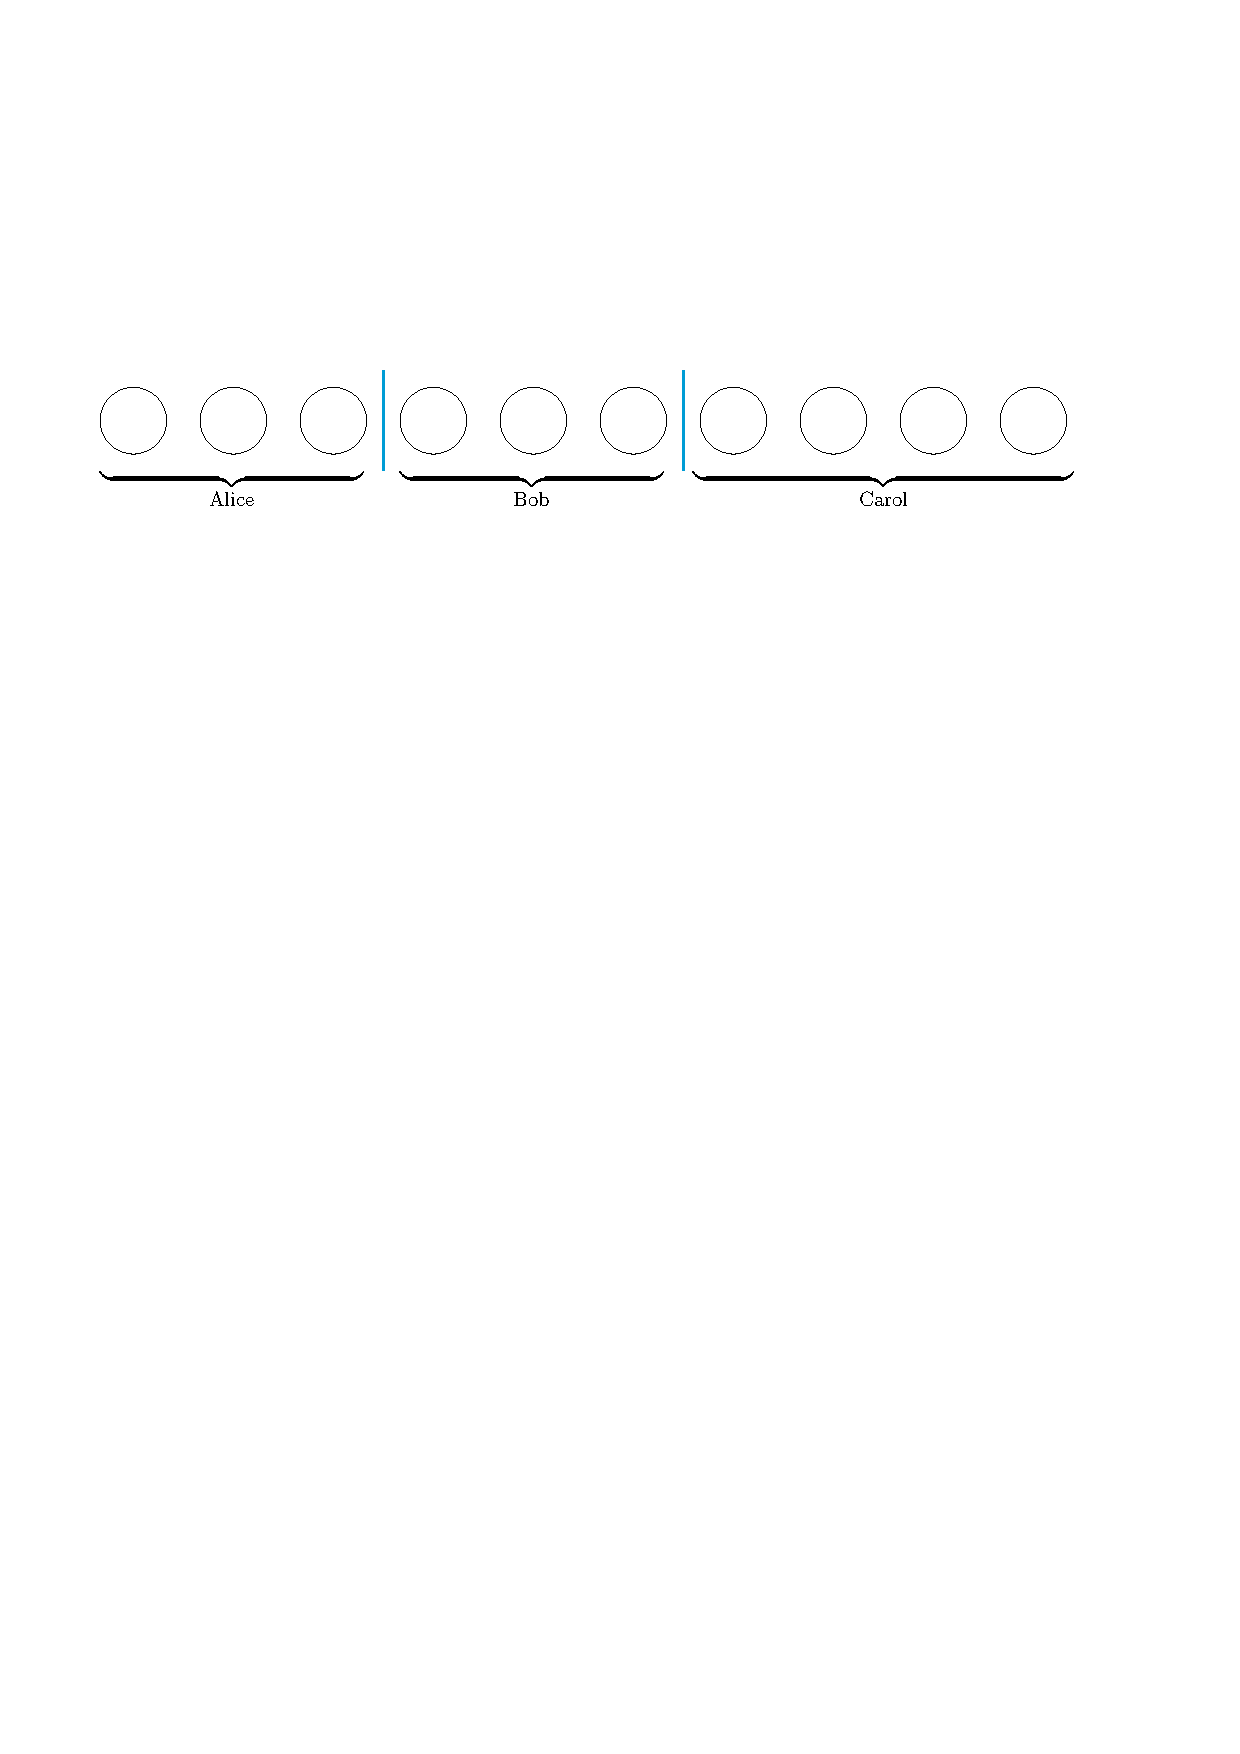
\includegraphics[width=.6\linewidth]{figures/cookie-distribution.pdf}
    \caption{Placing bars to partition the cookies.}
    \label{fig:cookie-distribution}
\end{figure}

In general, if there are $n$ identical items to be shared between $k \leq n$ people, then there are $\binom{n+(k-1)}{k-1}$ configurations. This method is known as the ``stars and bars'' method.

The cookie distribution example is equivalent to the question of asking how many integer solutions there are to the equation $x_1 + x_2 + x_3 = 10$, with the constraint $x_1,x_2,x_3 \geq 0$.

\textbf{Q}: Now, let us consider a variation of our pervious example. What if now we add the new constraint that \textbf{Alice and Bod each get at least 1 cookie}. \\
\textbf{A}: There are many ways to solve this modified example. One general way is to use \textit{\textbf{inclusion-exclusion}}. We eliminate cases where Alice gets 0 cookies and Bod gets 0 cookies. Then, add back the case where neither Alice nor Bob get cookies.

Alternatively, we can first distribution 2 cookies to Alice and Bob. For the remaining 8 cookies, we can distribute them as before.

\textbf{Q}: What if they can have cookies leftover? \\
\textbf{A}: Sum over all cases where they distribute $k$ cookies where $0 \leq k \leq 10$. Another easier way is to have ``\textbf{Charity}'' be the 4th person, so this is the number of ways 4 people are distributing 10 cookies. From this, we get
$$
\sum_{k=0}^{10} \binom{k+2}{2} = \binom{10 + 3}{3}
$$

\textbf{Q}: What if Alice wants at most 4 cookies? \\
\textbf{A}: Sum over cases where Alice gets $k$ cookies for $0 \leq k \leq 4$. Alternatively, subtract the number ways where Alice gets more than 4 cookies.

\begin{remark}
    For the previous example, we cannot assign 6 cookies to Bob and Carol and then distribute the rest 4. This results in double counting. Consider the following situations:
    \begin{itemize}
        \item Initially, give 3 cookies to Bob, 3 to Carol. Then give all 4 cookies to Bob.
        \item Initially, give 6 cookies to Bob, 0 to Carol. Then, give 1 to Bob and 3 to Carol.
    \end{itemize}
    Note that in both of these two situations, Alice, Bob, and Carol end up getting the same number of cookies. But the number of ways is counted twice.

    In combinatorics, it is always important to make sure that we don't overcount.
\end{remark}

\section{Lattice}

Recall the motivating example in the first lecture where we considered the ways to go from home to Bahen. We now generalize the problem into one concerning \textit{\textbf{lattice paths}}.

\begin{definition}[Lattice]
    An $m \times n$ grid between the coordinates $(0,0)$ and $(m,n)$ is called a \textit{\textbf{lattice}}.
\end{definition}

\begin{definition}[Lattice Path]
    A \textit{\textbf{lattice path}} for an $m \times n$ lattice between $(0,0)$ and $(m,n)$ is a sequence of ordered pairs of integers $(a_0,b_0),(a_1,b_1),\ldots,(a_t,b_t)$ such that for each $i$, $1 \leq i \leq t-1$ and either $(a_{i+1},b_{i+1}) = (a_i + 1, b_i)$ or $(a_{i+1},b_{i+1}) = (a_i, b_i + 1)$ (i.e. we can only move north or east by exactly one each step).
\end{definition}

A lattice path of length $t$ can be represented equivalently using a binary string of length $t-1$ over the alphabet $\{\mathrm{N,E}\}$.

\textbf{Q}: If we have a square lattice from $(0,0)$ to $(n,n)$, how many lattice paths from $(0,0)$ to $(n,n)$ do not go above the line $x=y$?

\begin{figure}[htbp]
    \centering
    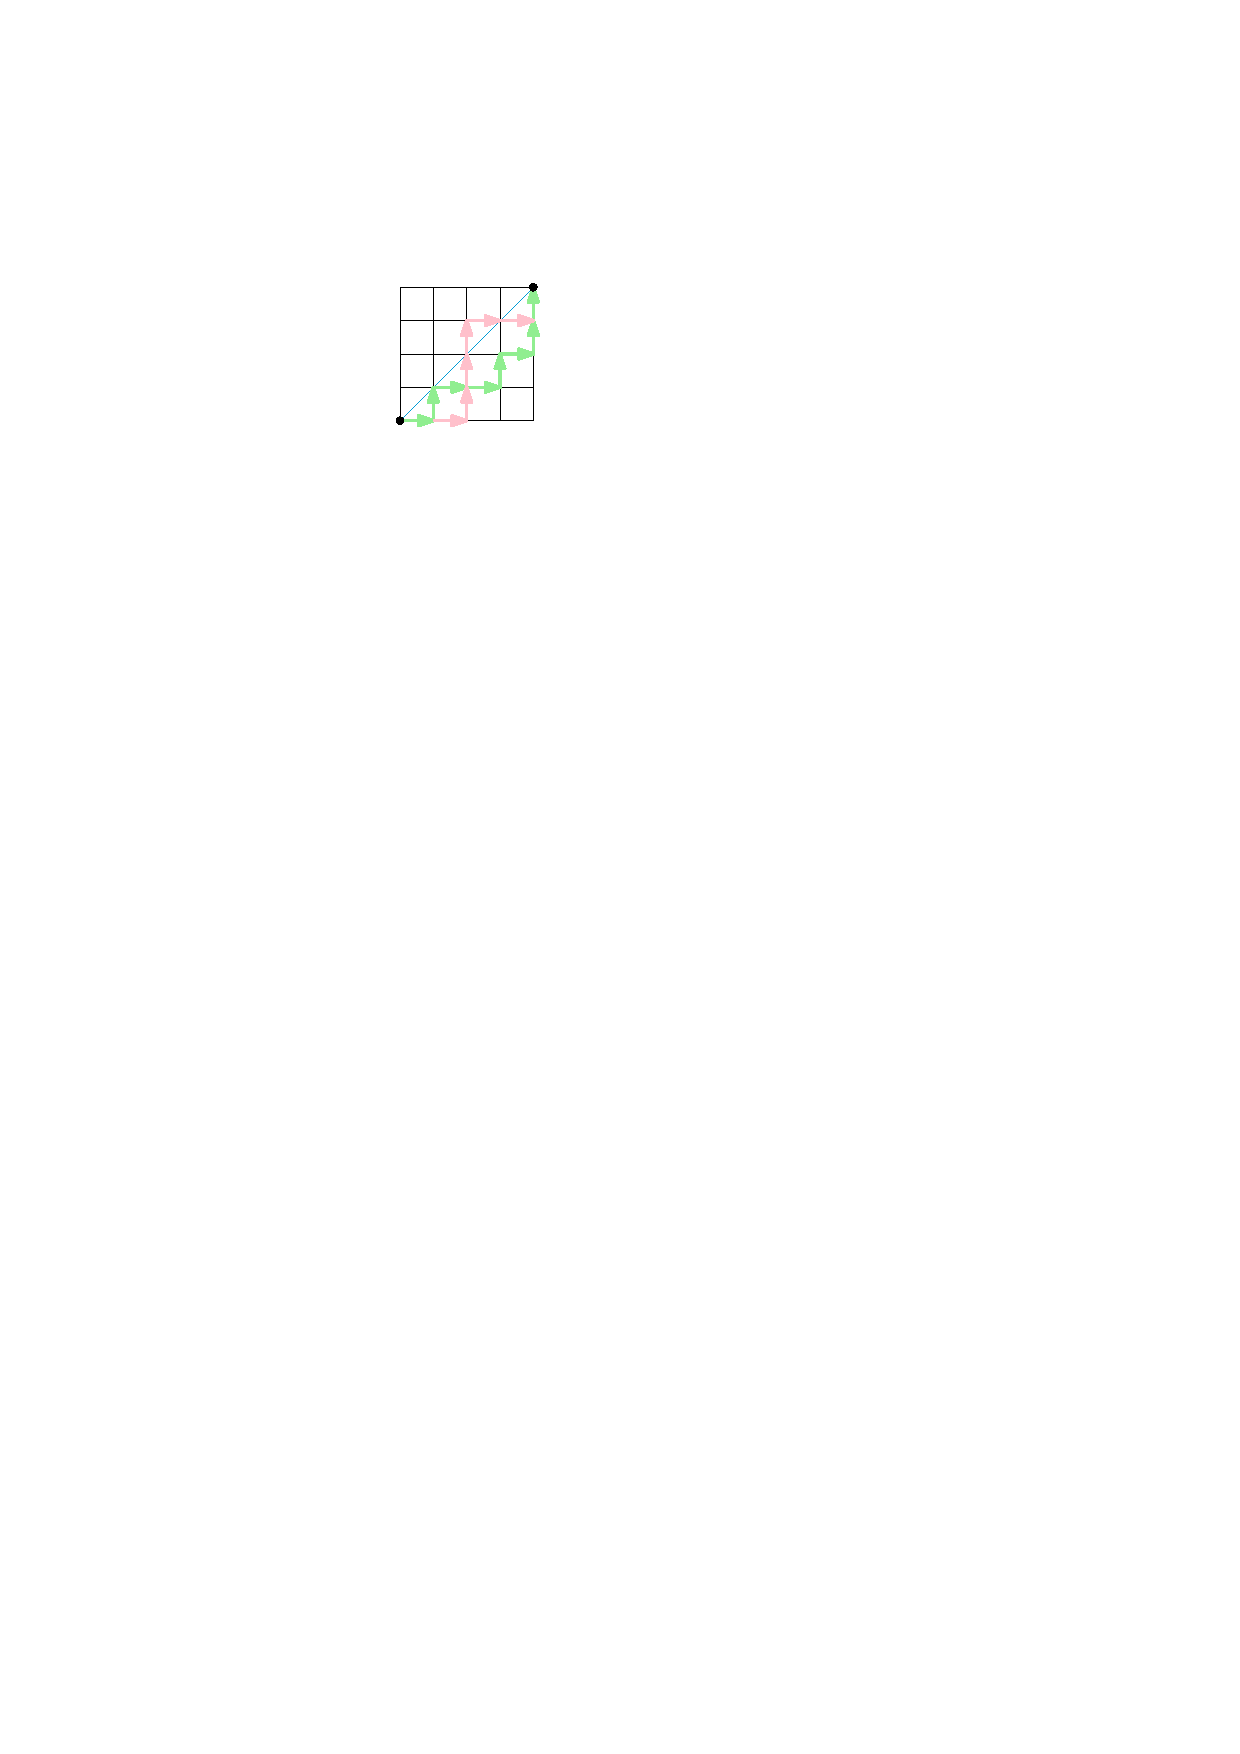
\includegraphics[width=.2\linewidth]{figures/dyck-path.pdf}
    \caption{The green path is a valid Dyck path whereas the red path is not.}
    \label{fig:dyck-path}
\end{figure}

\begin{definition}[Dyck Path]
    Lattice paths from $(0,0)$ to $(n,n)$ that do not go above the diagonal line $x=y$ are called \textit{\textbf{Dyck paths}} of length $2n$.
\end{definition}

Then, the $\{(,)\}$-string (string over the alphabet containing left and right parentheses, where ``('' corresponds to East, ``)'' corresponds to North) of length $2n$ that correspond to Dyck paths are exactly the strings where we do not have more ``)'' then ``('' as we read it from the left. Therefore, determining if a path is a Dyck path is equivalent to checking for \textbf{balanced parenthesis}.

We define the following notations
$$
\mathcal{L}_{(m,n)} = \{ \text{lattice paths from $(0,0)$ to $(n,n)$} \}
$$
and
$$
\mathcal{D}_{n} = \{ \text{Dyck paths of length $2n$} \}
$$

\begin{definition}[Catalan Number]
    The number of Dyck paths of length $2n$ is $C(n)$. $C(n)$ is called the $n$th \textit{\textbf{Catalan number}}.
\end{definition}

\begin{theorem}
    $$
    C(n) = \binom{2n}{n} - \binom{2n}{n-1}
    $$
\end{theorem}

\begin{remark}
    $$
    \begin{aligned}
        \binom{2n}{n} - \binom{2n}{n-1} &= \frac{(2n)(2n-1)\cdots (n+1)}{n(n-1)\cdots (1)} - \frac{(2n) \cdots (n+2)}{(n-1) \cdots (1)} \\
        &= \frac{(2n)(2n-1)\cdots (n+1)}{n(n-1)\cdots (1)} - \frac{(2n) \cdots (n+2){\color{red} n(n+1)}}{(n-1) \cdots (1) {\color{red} n(n+1)}} \\
        &= \frac{(2n)(2n-1) \cdots (n+1)}{(n)(n-1) \cdots (1)} \left[ 1 - \frac{n}{n+1} \right] \\
        &= \binom{2n}{n} \frac{1}{n+1}
    \end{aligned}
    $$
\end{remark}

\begin{proof}
    Let
    $$
    \mathcal{B}_{n} = \{ \text{lattice paths from $(0,0)$ to $(n,n)$ that go above $x=y$} \}
    $$
    be the set of non-Dyck paths. Then, $\mathcal{L}_{(n,n)} \setminus \mathcal{B}_n = \mathcal{D}_n$.

    Since $\mathcal{B}_n$ is a finite set, $|\mathcal{L}_{(m,n)} \setminus \mathcal{B}_n| = |\mathcal{L}_{(n,n)}| - |\mathcal{B}_n|$. We already know that $|\mathcal{L}_{(n,n)}| = \binom{2n}{n}$. This is from choosing $n$ positions to go North or $2n-n$ positions to go East.

    For $|\mathcal{B}_n|$, we would like to consider how to transform a ``bad'' lattice path into one that goes $n-1$ units E and $n+1$ units N. For a bad path, since it goes above the diagonal, there must be a first time it goes above $x=y$.

    Let $s = s_1s_2\ldots s_{2n}$ be a bad path. We claim that the first step when $s_i$ goes above $x=y$ is at an odd index $i$. This is because immediately before we crossed the line, we were on the line at index $i-1$ with $x=y$. At that point, we must have taken the same number of steps East as North. Up until $s_i$, we have used 1 more N than E. After $s_i$, there is one less N than E in the remaining steps.

    Consider the transformation 
    $$
    s_1s_2s_3\ldots s_i s_{i+1} \ldots s_{2n} \to s_1s_2s_3 \ldots s_i \overline{s_{i+1}} \ldots \overline{s_{2n}}
    $$
    We observe that this new path is a lattice path from $(0,0)$ to $(n-1,n+1)$. For that, there are $\binom{2n}{n-1}$ possible paths.

    Pictorially, we flip the steps after the $i$th move as shown in the figure below.

    \begin{figure}[htbp]
        \centering
        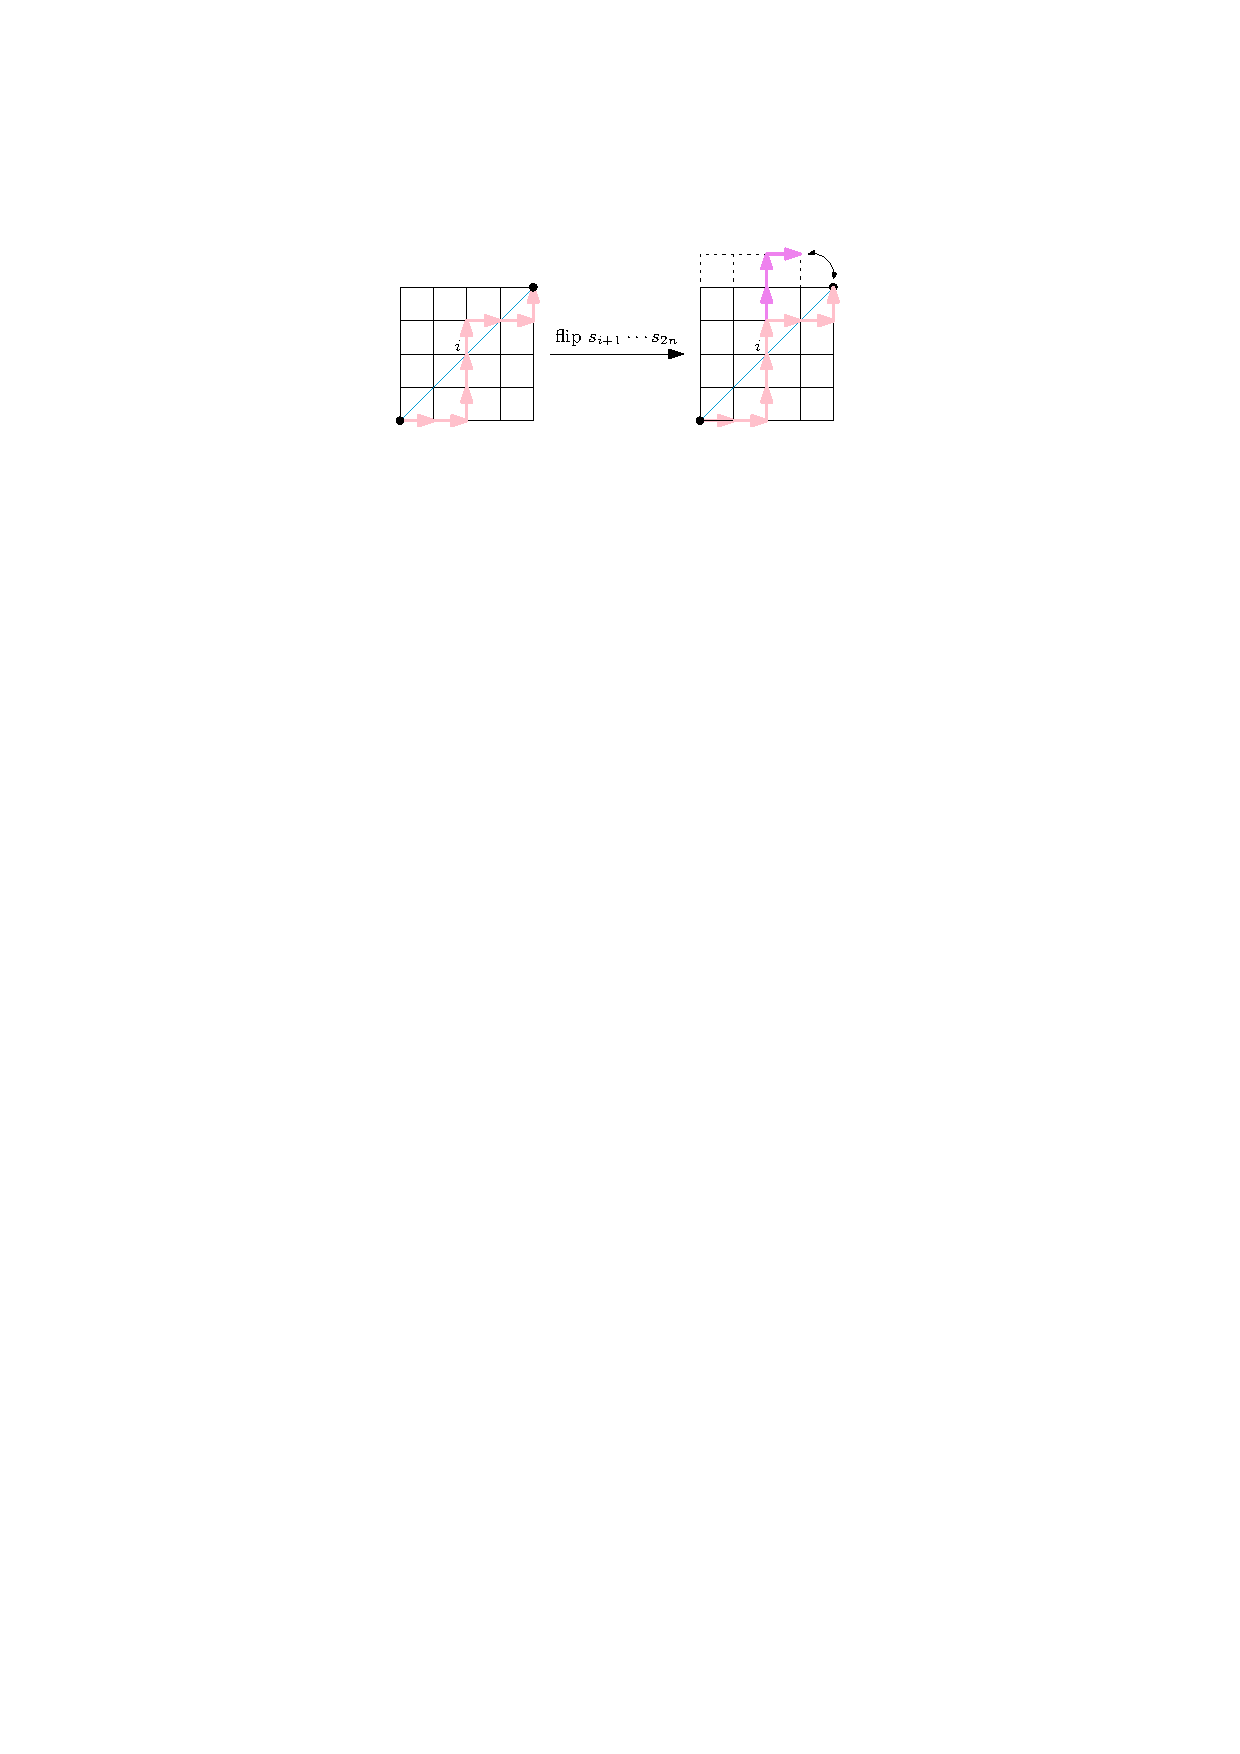
\includegraphics[width=0.5\linewidth]{figures/catalan-number-proof.pdf}
        \caption{Converting a non-Dyck path from $(0,0)$ to $(n,n)$ that goes above $x=y$ into a path in an $n-1 \times n+1$ lattice.}
        \label{fig:catalan-number-proof}
    \end{figure}
\end{proof}